% Chapter 1: INTRODUCTION

\chapter{Introduction} % Main chapter title

\label{introduction} % For referencing the chapter elsewhere, use \ref{Chapter1} 

%----------------------------------------------------------------------------------------

% Define some commands to keep the formatting separated from the content 
\newcommand{\keyword}[1]{\textbf{#1}}
\newcommand{\tabhead}[1]{\textbf{#1}}
\newcommand{\code}[1]{\texttt{#1}}
\newcommand{\file}[1]{\texttt{\bfseries#1}}
\newcommand{\option}[1]{\texttt{\itshape#1}}

%----------------------------------------------------------------------------------------


In the following chapter we will briefly familiarise the reader with the biological background of this work, summarise recent literature regarding the problem at hand to put our work into context and show in which way it contributed to the field.
%RELEVANCE AND TOPICALITY OF THE AIMS AND OBJECTIVES AND MY CONTRIBUTION TO THE RESEARCH.
%HOW HAS THE PROJECT ADVANCED THE FIELD?

%----------------------------------------------------------------------------------------
%----------------------------------------------------------------------------------------
\section{Biological background}

An important biological phenomenon studied by plant morphologists is \textit{tropism}, which is used to indicate the directional movement of a biological organism, here of a plant, when exposed to different environmental stimuli \cite{vandenbrink2014light}. Usually the stimulus involved is added to the name, e.g. \textit{phototropism} as a reaction to sunlight; it can be either \textit{positive}, i.e. towards the stimulus, or \textit{negative}, i.e. away from the stimulus. 
Various types of tropism are shown in figure \ref{fig:tropism}.

\begin{figure}[H]
	\centering
	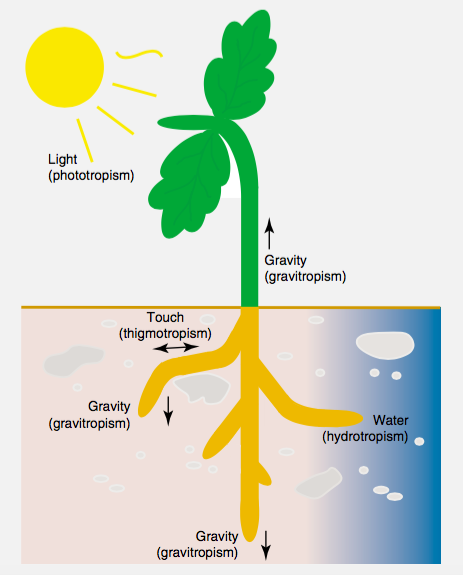
\includegraphics[width=0.6\textwidth]{../Figures/tropism.png}
	\caption{Different forms of tropism: Phototropism, thigmotropism, hydrotropism, and different effects of gravitropism; taken from \cite{gilroy2008plant}.}
	\label{fig:tropism}
\end{figure}

The most frequently observed and best studied tropism is \textit{gravitropism}, which describes the process of how plants grow as a response to gravity. It was firstly scientifically documented by Charles Darwin \cite{nick2017} and can be observed in many plants as well as other organisms: Roots show \textit{positive gravitropism}, i.e. they grow in the direction of the gravitational pull whereas stems grow in the opposite direction, see figure \ref{fig:tropism}. 
%An easy experiment to do is to lay a potted plant onto its side; over time the stem will begin to turn upwards and thus show negative gravitropism. 
\\
A far less studied process is \textit{electrotropism} which describes the growth or movement of a plant when exposed to an electric field (EF) and which is the tropism under study in this project. 

A high-overview explanation of the experimental setup and data collection to study electrotropism can be found in sections \ref{sec:data} and \ref{sec:experiment}.

%----------------------------------------------------------------------------------------
%----------------------------------------------------------------------------------------
\section{Literature review}

The majority of traditional root development bioassays only consider a small number of points \cite{parry2001novel,french2009high}. They are informative in terms of long-term effects on root growth; however, small and temporary changes can not be captured \cite{parry2001novel}.
Recently developed tools have considered a higher number of time points which allows a better study of how the growth process develops and the plant's responses \cite{french2009high,ishikawa1997novel,van2003new,chavarria2008spatio,miller2007computer}.

Image sequences can contain a representative "snapshot" description of a plant's developmental stage; also they can be generated at high speed (see section \ref{sec:experiment}). From manual time-lapse photography \cite{van1934einfluss,michener1938action} to measure lengths of seedlings after applying different external stimuli, digital camera  technology has improved and low digital storage cost has become available which has made it comparatively easy to collect large, time-stamped digital image data sets monitoring root growth \cite{french2009high}.
Once the root growth changes have been extracted from the image data, one can correlate their timing with the impact of different external signals including hormonal and environmental on processes such as cell division and cell expansion \cite{french2009high}. This will help us to understand root development in general. 

Analysing image data manually, however, is time-consuming, very subjective and thus error-prone \cite{french2009high}. When the analysis is done "by eye", it becomes difficult to reproduce measurements as they are not standardised by any automatised approach; the computations lack objectivity, and are subject to a significant human bias. Also, subtle phenotypes, such as a delay in the response, might be missed \cite{french2009high}. 
%Therefore, high-throughput software tools that can produce objective, quantitative analyses od the resulting images are now required.

Different groups have developed tools for gravitropism and have shown the power of automatised image-analysis techniques compared to manual methods. An overview was created in the appendix \ref{litreview}.


%----------------------------------------------------------------------------------------
%----------------------------------------------------------------------------------------
\section{Motivation}
The work described here is motivated by mainly three factors: definition and standardisation  or objectivity of the so far manually computed angle, flexibility and user-friendliness in the pre-processing step, and adaptability to standard consumer cameras. The software tool was designed to be used by a user, typically a biologist, with no need of specific knowledge in image processing nor plant morphology.

%----------------------------------------------------------------------------------------

%THIS NEEDS TO GO IN LITERATURE OVERVIEW
%\subsection{RootTrace}
%
%RootTrace [INSERT REFERENCE] has been developed to measure root lengths across time serie image data; biologists have also used it to measuer highly curved roots. A graphical user interface (GUI) implemented within the RootTrace framework makes it easy for the user to handle. However, this tool has failed on our image data set [INSERT REFERENCE HERE], probably due to the high noise level found in electrotropism images compared to gravitropism images.


%\subsection{PlantCV}
%
%COULD HAVE USED ONE OF THESE APPRAOCHES, BUT STARTED FROM SCRATCH. BASED ON THIS DATA SET.
%
%
%However, 
%Electopism much much harder since photos noisier.

